%%%%%%%%%%%%%%%%%%%%%%%%%%%%%%%%%%%%%%%%%
% University/School Laboratory Report
% LaTeX Template
% Version 2.0 (4/12/12)
%
% This template has been downloaded from:
% http://www.latextemplates.com
%
% License:
% CC BY-NC-SA 3.0 (http://creativecommons.org/licenses/by-nc-sa/3.0/)
%
% Original header:
%
% This is a LaTeX version of the sample laboratory report
% from Virginia Tech's copyrighted 08-09 CHEM 1045/1046 lab manual.
% Reproduction of this one appendix section for academic purposes
% should fall under fair use.
%
%%%%%%%%%%%%%%%%%%%%%%%%%%%%%%%%%%%%%%%%%

\documentclass{article}
\usepackage{graphicx}
\usepackage{float}
\usepackage{mathtools}

\title{ELEC 302-81\\ Lab 3\\ Non-Ideal Transformer Properties} % Title
% \author{John \textsc{Smith}} % Author name
\date{\today} % Specify a date for the report

\begin{document}

\maketitle

\begin{center}
  \begin{tabular}{lr}
    Date Performed: & February 4, 2013 \\
    Partners: & Rawley Dent \\
              & Charles Pittman \\
    Instructor: & Dr. Weatherford
  \end{tabular}
\end{center}

\pagebreak

%\setlength\parindent{0pt} % Removes all indentation from paragraphs

\section{Purpose of Experiment}

In this experiment, the non-ideal properties of a transformer were examined.
The performance of the transformer at the Lab-Volt station was first analyzed
by measuring the primary and secondary: voltages, currents, and powers. Then
the transformer was subjected to an open-circuit test and a short-circuit test
in order to generate the equivalent circuit components. These results were then
compared to the original performance specifications to show the transformer's
non-ideal properties.

\section{Procedure}

\subsection{EMS Workstation Set-up}

At the Lab-Volt EMS workstation, a Fluke multi-meter was used to measure the DC
resistance of the transformer windings. These values are recorded in
Table~\ref{tab:wind_res}.  The DAI 24V supply was turned on, and the DAI USB
connector was connected between the EMS workstation and the {PC}. On the LVDAM
EMS application software, the metering windows for E$_1$, E$_2$, I$_1$, and
I$_2$ were opened, set to continuous refresh.

\subsection{Transformer Performance}

\label{part1} With the main power switch set OFF and the voltage control knob
fully CCW, the voltmeter selector switch was set to position 4--N. The circuit
represented by Figure~\ref{fig:circuit_01} was constructed with the secondary
voltmeter E$_2$ open-circuited at first to simulate an infinite load.  The main
power supply was turned on, and the supply voltage was adjusted to {120V}. The
primary voltage E$_1$, primary current I$_1$, input power P$_1$, secondary
voltage E$_2$, secondary current I$_2$, and output power P$_2$ were then
measured for each of the four different loads listed in
Table~\ref{tab:voltage_rat}.  Prior to changing each load, the voltage supply
knob was set fully CCW and the main power switch to OFF.

\subsection{Open Circuit Test}

\label{part2} The circuit shown in Figure~\ref{fig:circuit_02} was then constructed. The main power switch
was set ON and the voltage control knob was adjusted to 120V. The values of the primary voltage E$_1$, primary
current I$_1$, and input power P$_1$ were measured. These values were recorded in Table~\ref{tab:open_circ}.
The main power switch was set OFF and the voltage control knob fully CCW.

\subsection{Short Circuit Test}

\label{part3} The circuit shown in Figure~\ref{fig:circuit_03} was then constructed. It was noted that 
I$_2$ short circuited the secondary windings 5-6. Thus the voltage supply knob was slowly adjusted until
a secondary current of 0.4A was obtained. The primary voltage, primary current, input power, and the 
secondary current were measured. These values were recorded in Table~\ref{tab:short_circ}.
The main power switch was set OFF and the voltage control knob fully CCW.

\section{Results}
\subsection{Transformer Performance}
\begin{table}[H]
  \centering
  \begin{tabular}{*{2}{c}}
    \textbf{Winding} & \textbf{Resistance} \\
    \textbf{\#} & $\Omega$ \\
    \hline
    1--2 &  7.9 \\
    5--6 &  7.9 \\
  \end{tabular}
  \caption{Winding Resistances}
  \label{tab:wind_res}
\end{table}

\begin{table}[H]
  \centering
  \begin{tabular}{*{7}{c}}
    & \multicolumn{2}{c}{\textbf{Primary}} & \textbf{Input}
    & \multicolumn{2}{c}{\textbf{Secondary}} & \textbf{Output} \\
    \textbf{Load} & \textbf{Voltage} & \textbf{Current} & \textbf{Power}
    & \textbf{Voltage} & \textbf{Current} & \textbf{Power} \\
    Z$_\text{L}$ $\Omega$ & E$_1$ V & I$_1$ A & P$_1$ W
    & E$_2$ V & I$_2$ A &
    P$_2$ W \\
    \hline
    $\infty$   & 119.9 & 0.027 & 2.453 & 119.0 & 0.003 & 0 \\
    300        & 119.3 & 0.388 & 46.01 & 112.4 & 0.368 & 41.35 \\
    300 + j300 & 119.5 & 0.270 & 23.63 & 112.4 & 0.244 & 20.20 \\
    300 - j300 & 119.5 & 0.281 & 27.30 & 120.0 & 0.276 & 23.52 \\
  \end{tabular}
  \caption{Primary and secondary voltages and currents}
  \label{tab:volt_rat}
\end{table}

\subsection{Open Circuit Test}
\begin{table}[H]
  \centering
  \begin{tabular}{*{3}{c}}
    \multicolumn{2}{c}{\textbf{Primary}} & \textbf{Input} \\
    \textbf{Voltage} & \textbf{Current} & \textbf{Power} \\
    E$_1$ V & I$_1$ A & P$_2$ W \\
    \hline
    119.7 & 0.027 & 2.44 \\
  \end{tabular}
  \caption{Open Circuit}
  \label{tab:open_circ}
\end{table}

\subsection{Short Circuit Test}
\begin{table}[H]
  \centering
  \begin{tabular}{*{4}{c}}
    \multicolumn{2}{c}{\textbf{Primary}} & \textbf{Input} & \textbf{Secondary} \\
    \textbf{Voltage} & \textbf{Current} & \textbf{Power} & \textbf{Current} \\
    E$_1$ V & I$_1$ A & P$_1$ W & I$_2$ A \\
    \hline
    11.7 & 0.403 & 2.607 & 0.398 \\
  \end{tabular}
  \caption{Data for Fig~\ref{fig:circuit_03}}
  \label{tab:short_circ}
\end{table}

\section{Analysis}
\subsection{Transformer Equivalent Circuit Component Values}
\begin{table}[H]
  \centering
  \begin{tabular}{*{4}{c}}
    \textbf{R$_C$} & \textbf{X$_M$} & \textbf{R$_{eq}$} & \textbf{X$_{eq}$} \\
    $\Omega$ & $\Omega$ &$\Omega$ & $\Omega$ \\
    \hline
    5.85k & 6.80k & 16.05 & 24.19 \\
  \end{tabular}
  \caption{Equivalent Transformer Components}
  \label{tab:equiv_comp}
\end{table}

\subsection{Transformer Losses}
\begin{table}[H]
  \centering
  \begin{tabular}{*{3}{c}}
    & \multicolumn{2}{c}{\textbf{Losses}} \\
    \textbf{Load} $\Omega$ & \textbf{P$_\text{Cu}$} W & \textbf{P$_\text{core}$} W \\
    \hline
    $\infty$ & 0.0014 & 2.453 \\
    300 & 2.162 & 2.433 \\
    300 + j300 & 0.956 & 2.441 \\
    300 - j300 & 1.223 & 2.437 \\
  \end{tabular}
  \caption{Copper and Core Losses}
  \label{tab:power_losses}
\end{table}

\subsection{Voltage Regulation and Efficiency Comparison}
\begin{table}[H]
  \centering
  \begin{tabular}{*{4}{c}}
    \textbf{Load} $\Omega$ & \textbf{VR} & \textbf{VR} & \textbf{Percent} \\
    & Part 1 & R$_\text{eq}$ & \textbf{Difference} \\
    \hline
    $\infty$ & 0.00 & 0.00 & 0.00 \\
    300 & 5.97 & 6.39 & 7.0 \\
    300 + j300 & 6.16 & 6.69 & 8.6 \\
    300 - j300 & -0.92 & -1.25 & 35.9 \\
  \end{tabular}
  \caption{Transformer Voltage Regulation (VR)}
  \label{tab:vr}
\end{table}

\begin{table}[H]
  \centering
  \begin{tabular}{*{4}{c}}
    \textbf{Load} $\Omega$ & $\eta$ & $\eta$ & \textbf{Percent} \\
    & Part 1 & R$_\text{eq}$ & \textbf{Difference} \\
    \hline
    $\infty$ & 0.00 & 0.00 & 0.00 \\
    300 & 89.72 & 87.41 & 2.6 \\
    300 + j300 & 85.57 & 86.02 & 0.5 \\
    300 - j300 & 86.11 & 86.93 & 0.9 \\
  \end{tabular}
  \caption{Transformer Efficiencies ($\eta$)}
  \label{tab:eff}
\end{table}

\section{Conclusions}

By measuring the resistance of each transformer winding and not getting any
extremely high resistance readings similar to an open circuit, it was
determined that the transformer windings had no faults and the integrity of the
windings were intact.

In Table~\ref{tab:equiv_comp} the circuit components of the transformer equivalent circuit are listed. These
values were computed by using the voltage, current, and power values obtained from both the open-circuit
test and short-circuit test. 

In Table~\ref{tab:power_losses} the copper and core losses for each load are listed. The copper loss equation
used was P$_Cu$ = I$_S$


\section*{Circuits Tested}
\begin{figure}[H]
  \centering
  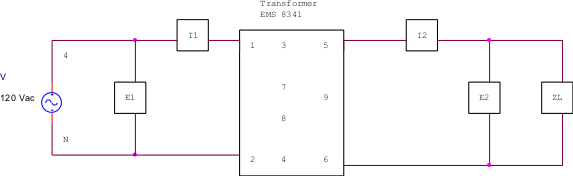
\includegraphics[width=.8\textwidth]{img/circuit_01}
  \caption{Single Phase Transformer Circuit for part one}
  \label{fig:circuit_01}
\end{figure}

\begin{figure}[H]
  \centering
  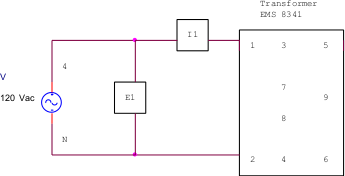
\includegraphics[width=.8\textwidth]{img/circuit_02}
  \caption{Single Phase Transformer Circuit for part two (open circuit test)}
  \label{fig:circuit_02}
\end{figure}

\begin{figure}[H]
  \centering
  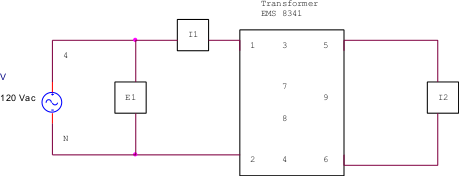
\includegraphics[width=.8\textwidth]{img/circuit_03}
  \caption{Single Phase Transformer Circuit for part two (short circuit test)}
  \label{fig:circuit_03}
\end{figure}

\end{document}
